\documentclass[mathserif, aspectratio=169]{beamer}


\usepackage{movie15}
\usepackage{psfrag,graphicx}
\usepackage{amsmath}
\graphicspath{{figs/}}

\usetheme{Boadilla}
\makeatother
\setbeamertemplate{footline}[frame number]

\usepackage{graphicx}
\usepackage{caption}
\usepackage{subcaption}
\captionsetup{compatibility=false}
\usepackage{amsmath} 
\usepackage{amssymb} 
\usepackage{amsthm}  
\usepackage{bm}
\usepackage{lipsum}
\usepackage[linesnumbered, ruled]{algorithm2e}
\usepackage{color}
\newtheorem{assumption}{Assumptions}
\newtheorem{prop}{Proposition}
\newtheorem{defn}{Definition}
\newtheorem{thm}{Theorem}
\newtheorem{lem}{Lemma}
\newtheorem{cor}{Corollary}
\newtheorem{sol}{Decentralized Solution}
\newtheorem{thresh}{$\epsilon$-thresholding}
\definecolor{light-gray}{gray}{0.8}
\usepackage{textcomp}

\newcommand{\backupbegin}{
   \newcounter{finalframe}
   \setcounter{finalframe}{\value{framenumber}}
}
\newcommand{\backupend}{
   \setcounter{framenumber}{\value{finalframe}}
}
\newcommand{\norm}[1]{\left\lVert #1 \right\rVert}

\makeatletter
\setbeamertemplate{navigation symbols}{}


\title[Lecture 19] % (optional, use only with long paper titles)
{Data, Environment and Society: \\{Lecture 19: Model Selection and Regularization}}


%\subtitle
%{Include Only If Paper Has a Subtitle}

\author[ER190C: Data, Environment and Society] 
{Instructor: Duncan Callaway\\
GSI: Seigi Karasaki} 
% - Give the names in the same order as the appear in the paper.
% - Use the \inst{?} command only if the authors have different
%   affiliation.

%\logo{
%\includegraphics[width=1.5cm,height=1.5cm,keepaspectratio]{uvic_logo_h.jpg}
%}
\vspace{-20mm}
\institute[UC Berkeley] % (optional, but mostly needed)
 {\small{ \bf October 25, 2018}}


\date[October 25, 2018]

\begin{document}

\frame{
  \titlepage
}

\begin{frame}{Introduction}
We've been working a lot with this model:

\begin{equation*}
Y = \beta_0+\beta_1X_1+\cdots+\beta_pX_p+\epsilon
\end{equation*}\\~\\
And we know well how to fit it with least squares regression.\\~\\

Today's topic: how can we improve on the ``standard'' strategy of choosing coefficients via a one step application of least squares regression?\\~\\
\end{frame}

\begin{frame}{Stop using OLS?  Wait, why improve on a good thing?}
Let $n=$ number of observations, and $p=$ number of features.
 \begin{enumerate}
\item When $n$ close to $p$ in size, least squares fit can have high variance $\rightarrow$ overfitting.
\begin{itemize}
\item As we'll see, some model fitting methods are naturally good at reducing variance (but at a small bias penalty)
\end{itemize}
\item When $p$ is big, if every variable gets a coefficient it can be hard to interpret models.  
\begin{itemize}
\item A subset of model selection known as ``feature selection'' helps get rid of some features.
\item This lets you ``throw in the kitchen sink'' with the faith that the feature selection process will get rid of it if it's not helping.
\end{itemize}
\end{enumerate}
\end{frame}

\begin{frame}{Ok, how do you do it?}
We'll look at two kinds of methods in Ch 6 (today and next Tuesday):
\begin{itemize}
\item Subset selection -- today
\item Shinkage -- today and tuesday
\end{itemize}

{\large \color{blue} Today's Objectives}
\begin{itemize}
\item Refine our understanding of model identification as an optimization problem
\item Learn how to adjust your errors to compare models with different numbers of predictors
\item Understand what ``regularization'' is and why we do it
\item Understand the tradeoffs between subset selection, ridge regression, and lasso
\end{itemize}


\end{frame}

\begin{frame}{Aside: $n$ choose $k$}
To aid in discussing the process it helps to understand the formula for binomial coefficients.\\~\\

When we are choosing $k$ things from a group of $n$, this formula tells us how many unique combinations of $k$ things there are.

\begin{equation}
{{n}\choose{k}} = \frac{n!}{k!(n-k)!}
\end{equation}

Simple examples:  

\begin{align*}
{{3}\choose{2}} &= \uncover<2->{\frac{3!}{2!(1!)} = 3\text{, where the set is } {(1,2), (1,3), (2,3)}}\\
{{4}\choose{2}} &= \uncover<2->{\frac{4!}{2!(2!)} = 6\text{, where the set is } {(1,2), (1,3), (1,4), (2,3), (2,4), (3,4)}}
\end{align*}
\end{frame}

\begin{frame}{How many models?}

Say you have $p$ features and want to construct as many unique linear models as you can with just $k$ features.  \\~\\

How many models are there?\\

\pause

\begin{align*}
{p\choose{k}} = \frac{p!}{k!(p-k)!}
\end{align*}

\end{frame}

\begin{frame}{``Best'' subset selection}

1. Find $\mathcal{M}_0$ = model with $p=0$ (just a constant term...will be equal to the mean)\\~\\

2. Define $\mathcal{M}_k$ = the best model with $k$ predictors, chosen from among the $p\choose{k}$ models with $k$ predictors.  Choose ``best'' via something like $R^2$.  Find $\mathcal{M}_k$ for all $k$, using all the training data.\\~\\

3. Then use a model selection method like k-fold cross validation (or other adjusted error approaches like AIC, $C_p$, to be discussed) to choose from among $\mathcal{M}_0,\cdots\mathcal{M}_p$.

\end{frame}

\begin{frame}{When to cross-validate or use an adjusted error?}

\textbf{Question}:  Why could we just use $R^2$ with all the training data for step two, but not step three?

\vspace*{3mm}

\pause
\textbf{Answer:} Error adjustment methods are needed to avoid overfit -- i.e. to keep you from using too many parameters.  If you're choosing from among a set of models that all have the same number of parameters (step two), you don't need to adjust.

\end{frame}


\begin{frame}{Is the perfect the enemy of the good?}

The ``best'' subset selection procedure is effective -- it guarantees you'll find \textit{the best} model.\\~\\

But it's not always practical to implement.  Why?

\pause

\begin{itemize}
\item Computing time!  You'd need to test 1 trillion models if you had $p=40$.
\end{itemize}

The alternatives: ``hueristic'' algorithms that give you a strategy to search the space of models but don't guarantee that you'll get the best model.  

\vspace{5mm}

\textit{Stepwise selection} (forward selection and backward selection) can help here.
\end{frame}


%\begin{frame}
%$\mathcal{M}_0\quad \mathcal{M}_1 \quad \mathcal{M}_2 \quad \mathcal{M}_3 \quad\mathcal{M}_4$
%
%\vspace{10mm}
%
%${{4}\choose{0}}=1\quad{{4}\choose{1}}=4\quad{{4}\choose{2}}=6\quad{{4}\choose{3}}=4\quad{{4}\choose{4}}=1$
%
%\end{frame}

\begin{frame}{Stepwise selection: Forward Selection}

\begin{columns}
\column{0.5\textwidth}

\textbf{Forward selection:} Start with $\mathcal{M}_0$.  Then to choose the best model from each higher ``level'':

\vspace{5mm}
\textit{First, }within each level, add one predictor at a time to the best model from the lower level.  Use $R^2$ or other to find the best model from this set of $\mathcal{M}_{k-1} \text{``}+ 1\text{''}$

\vspace{5mm}

\textit{Second,} choose from your list $\{\mathcal{M}_0, \mathcal{M}_1,...\mathcal{M}_{p}\}$ via cross validation or adjusted error metrics.\\~\\

\column{0.5\textwidth}

\vspace*{-15mm}
\begin{center}
\only<1>{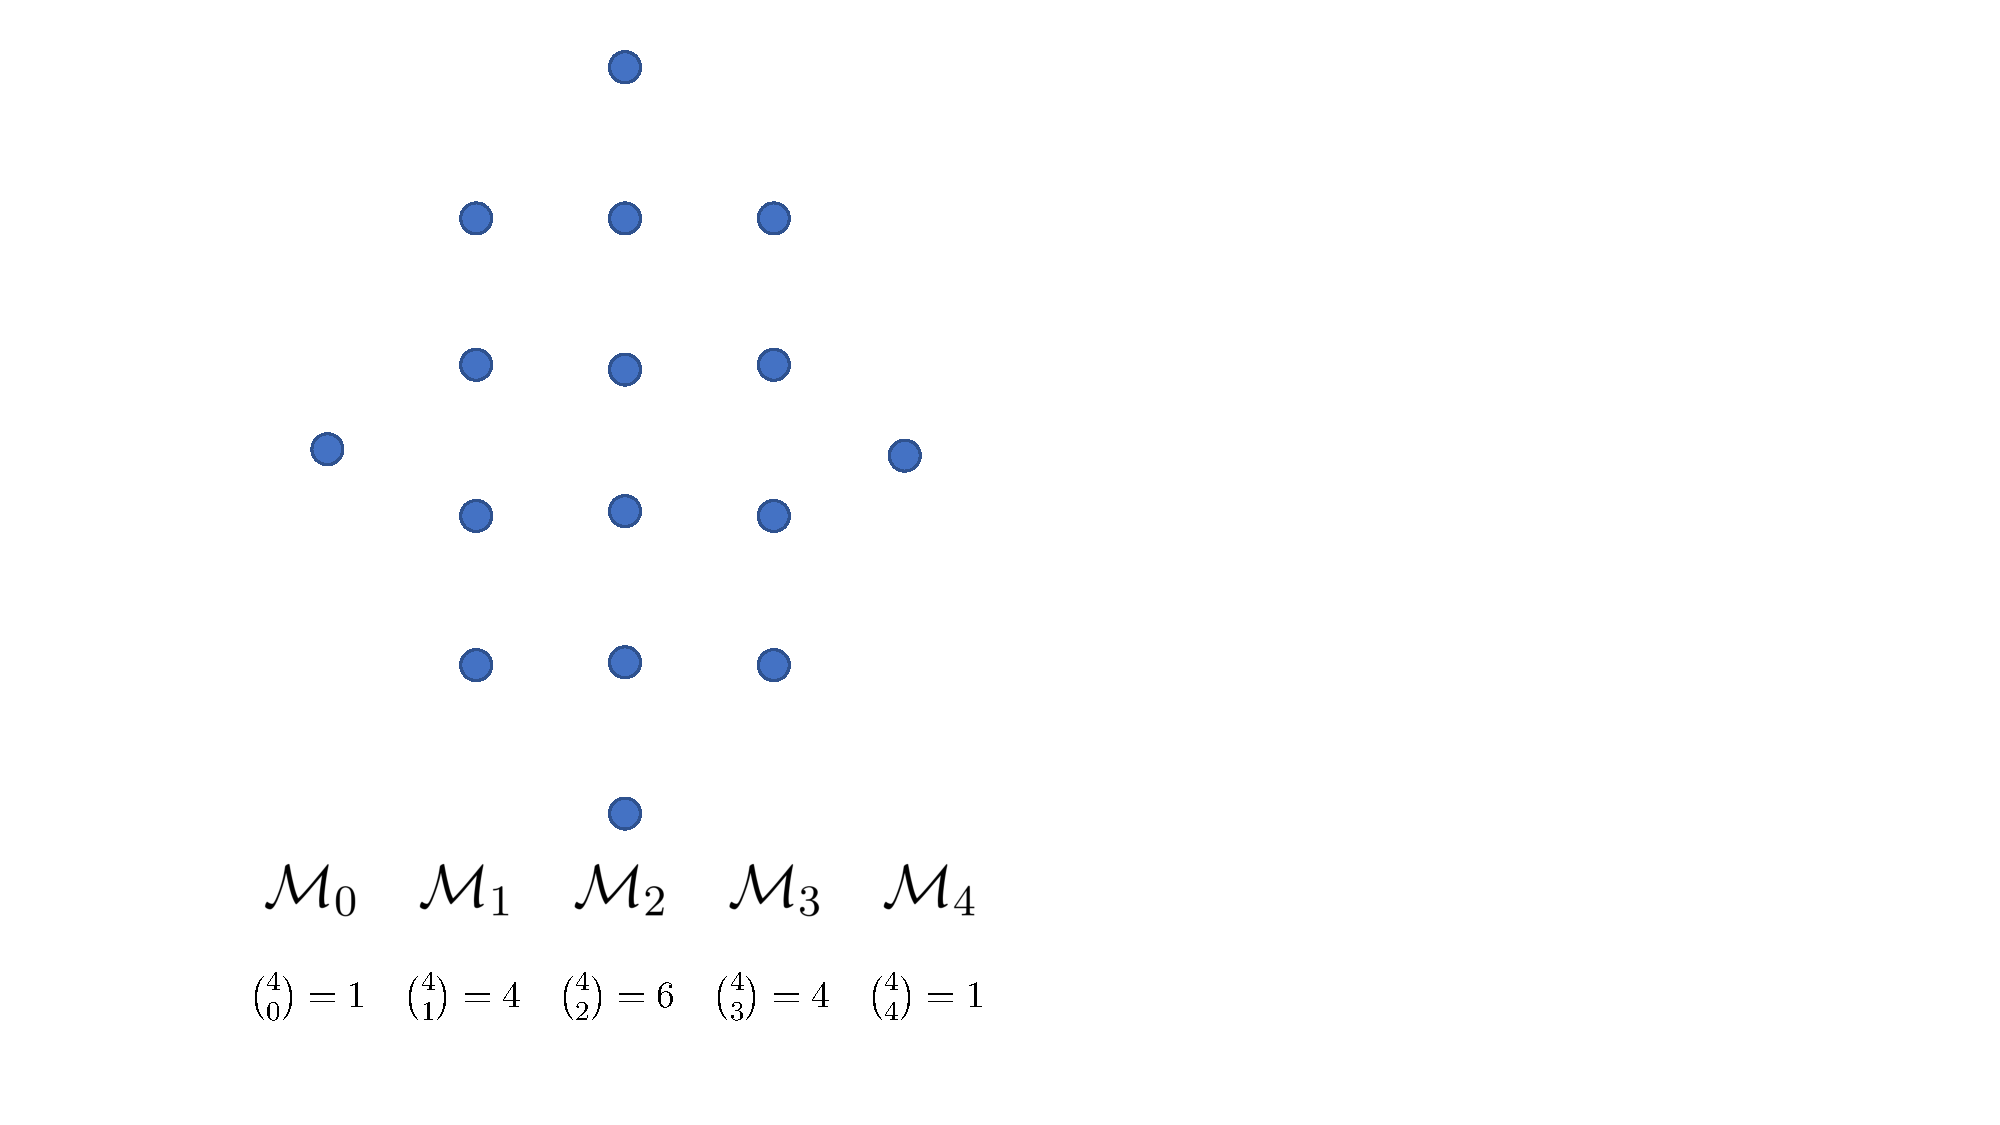
\includegraphics[scale=0.425]{4choosek_blank}}
\only<2>{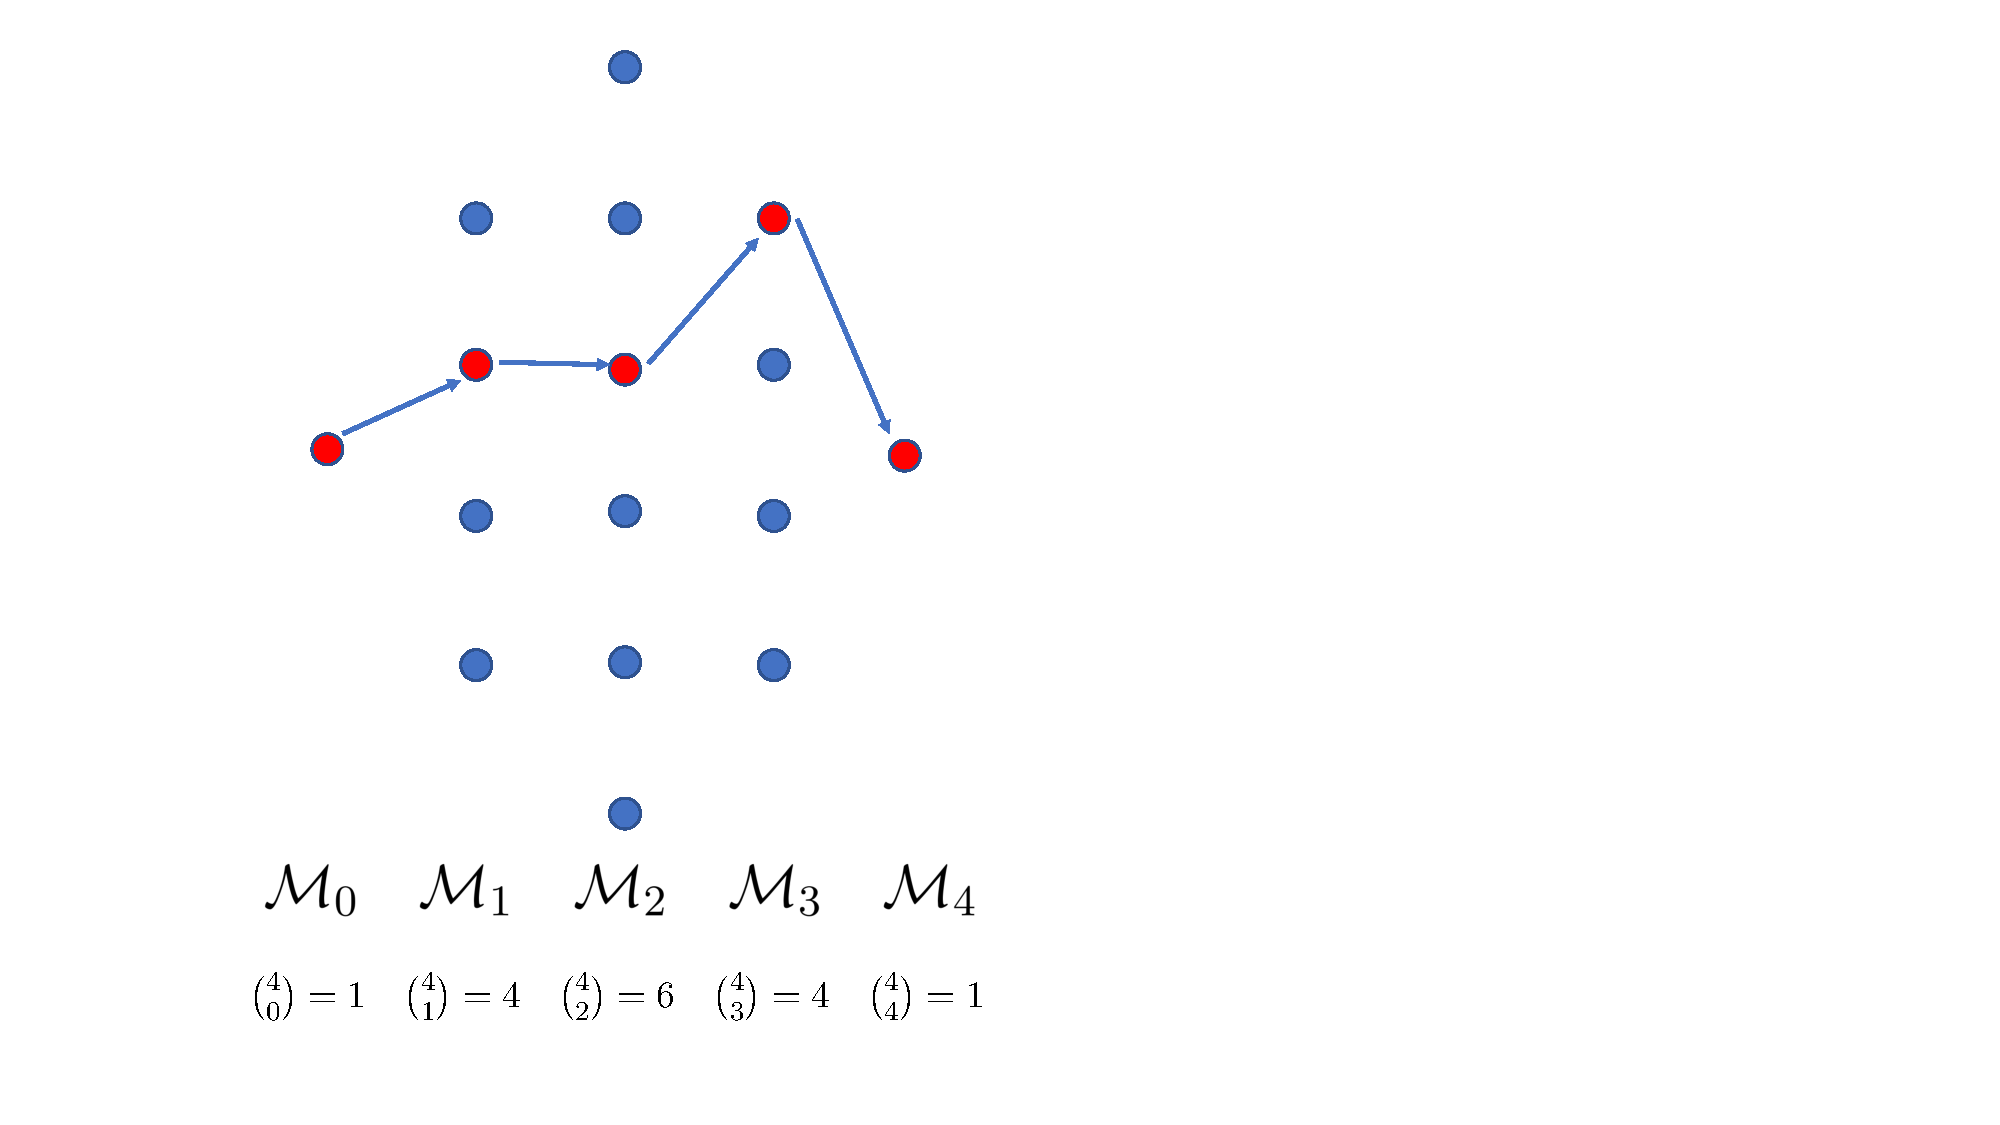
\includegraphics[scale=0.425]{4choosek_filled}}
\end{center}
\end{columns}

\end{frame}

\begin{frame}{Why is Forward Selection better than Best Subset Selection?}

\pause

...because we build on the best model from the lower level ($\mathcal{M}_{k-1}$)

\vspace{5mm}

How many models will we evaluate on each level?
\pause 

\vspace{5mm}

...For each level we are only choosing from $p-k$ possible models.  

\vspace{5mm}

Example:  suppose $p = 10$.  
\begin{itemize}
\item Best subset: evaluate $2^p = 1024$ models
\item Forward: evaluate $1 + 10 + 9 + 8 + 7 + ... + 1 = 56$ models
\end{itemize}



\end{frame}

\begin{frame}{Stepwise selection: Backward  Selection}

\pause
\textbf{Backward selection:} like forward selection, except that you start with $\mathcal{M}_p$ (the model with all predictors) and \textit{remove} one predictor at a time.

\end{frame}


\begin{frame}{Pop quiz}
\textbf{Challenge question:} which stepwise selection approach works in situations where $n<p$?\\~\\

\pause

\textbf{Answer:} Forward selection\\~\\

\pause

...because it naturally stops at models with $k=n-1$. 

\end{frame}

\begin{frame}{Tracing the best model}


\begin{figure}
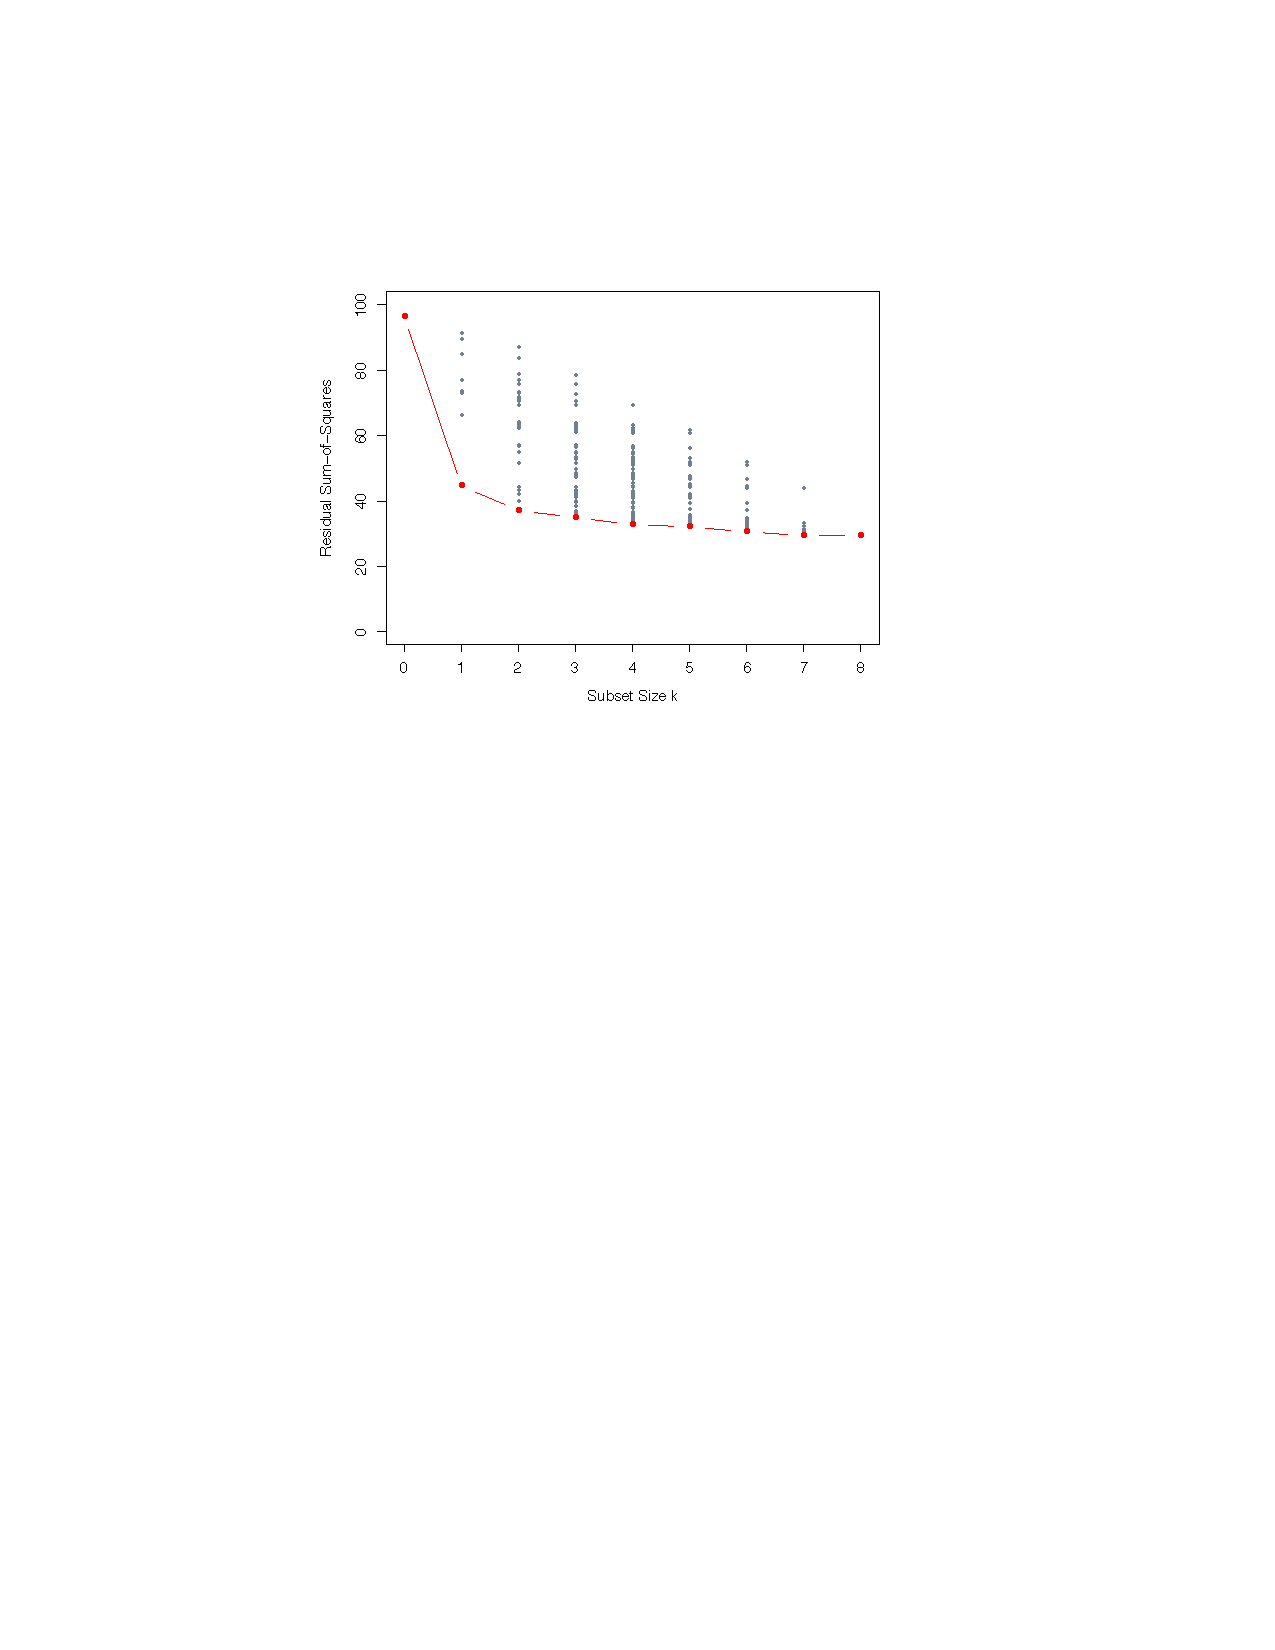
\includegraphics[scale=0.6]{subset_surfing}
\caption*{\tiny From Elements of Statistical Learning}
\end{figure}

Dots are performance for each possible model\\~\\

Red line is the performance for the best model in each subset size group.\\~\\

Stepwise selection would either ride on the red line or above.  
\end{frame}

\begin{frame}{Choosing from among models with different $k$}

As you increase the number of predictions in a model, \textit{training} data set error will naturally improve.  \\~\\\

But this might be in part due to over-fit, i.e. soaking up irreducible error with predictors that are are spuriously correlated with the error. \\~\\

Two approaches to deal with this problem:

\begin{enumerate}
\item Cross validation (see Ch 5 and notes from Class 18)
\item ``Adjust'' the errors with $C_p$, AIC, BIC or ``Adjusted $R^2$''
\end{enumerate}

\end{frame}



\begin{frame}{Shrinkage methods (regularization)}

Let's begin by remembering that the processes of choosing parameters \textit{and} choosing models are rooted in ideas of optimization.\\~\\

When we run OLS, we are solving a formal optimization problem

\begin{align*}
Y &= \beta_0+\beta_1X_1+\cdots+\beta_p X_p+\epsilon & Y_i &= \sum_{k=1}^{K} X_{ik} \cdot \beta_k +\epsilon_i
\end{align*}

\begin{align*}
\Rightarrow \hat{\beta}_\text{ols} = \text{arg }\min_\beta \sum_{i=1}^N \left(Y_i - X_i \beta \right)^2
\end{align*}

To solve, set the derivatives wrt $\beta$s to zero and 

\begin{align*}
\hat{\beta}_\text{ols} &= \left(\mathbf{X}^T\mathbf{X}\right)^{-1} \left(\mathbf{X}^T\mathbf{Y}\right)
\end{align*}

\end{frame}

\begin{frame}{Subset selection as optimization}

In subset selection, you can show that you're running this optimization model:

\begin{align*}
\hat{\beta}_{SS} = \arg \min_\beta \sum_{i=1}^N \left(Y_i - X_i \beta \right)^2+\lambda \cdot \norm{\beta}_0\text{, where }\norm{\beta}_0=\sum_{k=1}^K I(\beta_k)
\end{align*}

Here, $\norm{\cdot}_0$ is the ``zero norm,'' where $I(\cdot)$ is the `indicator function':

\begin{align*}
I(\beta)=
\begin{cases}
  1 & \text{for }\beta \ne 0\\    
  0 & \text{for }\beta = 0    
\end{cases}
\end{align*}

Note that the choice of $\lambda$ would correspond to using different error adjustments, e.g. 

\begin{align*}
\lambda = 2\hat{\sigma}
\end{align*}

for AIC and $C_p$.
\end{frame}

\begin{frame}{Subset selection as optimization, ctd}
For those of you with experience with integer programming
\begin{itemize}
\item The formulation on the last slide is a mixed integer quadratic program
\item There are solvers for this type of problem, so you don't have to take the heuristic approaches (forward selection, etc) if you don't want to.
\end{itemize}
\end{frame}

\begin{frame}{Ridge regression}
In ridge regression, we use a very intuitive objective function:

\begin{align*}
\hat{\beta}_{\text{ridge}} &= \arg \min_\beta \sum_{i=1}^N \left(Y_i - X_i \beta \right)^2+\lambda \cdot \sum_{k=1}^K \beta_k^2\\
&= \arg \min_\beta \sum_{i=1}^N \left(Y_i - X_i \beta \right)^2+\lambda \cdot ||\beta||_2^2 
\end{align*}

This leads to:

\begin{align*}
\hat{\beta}_\text{ridge} &=\left(\mathbf{X}^T\mathbf{X} + \lambda\mathbf{I}_k\right)^{-1} \left(\mathbf{X}^T\mathbf{Y}\right)
\end{align*}

Here 
\begin{itemize}
\item $\lambda$ is a tuning parameter -- it is not unique.  
\item $\mathbf{I}_k$ is the $k\times k$ identity matrix\\~\\
\end{itemize}

\textbf{Important}! Ridge regression produces different $\beta$ estimates for different choices of $\lambda$.

\end{frame}

\begin{frame}{Ridge regression advantages}

\pause

\textbf{First}.  Suppose some of your features are linear combinations of the others.  That means you can write $x_{i,j} = Ax_{i,-j}$ for at least 1 value of $j$. \\~\\

Then $\mathbf{X}^T\mathbf{X}$ is not ``full rank'' and you can't invert it.  I.e., $(\mathbf{X}^T\mathbf{X})^{-1}$ doesn't exist.

\begin{align*}
\text{e.g., }\mathbf{X}^T\mathbf{X} = 
\begin{bmatrix}
1 & 2 & 3\\
2 & 4 & 6\\
3 & 6 & 9
\end{bmatrix}
\uncover<3->{\text{ \quad vs.  \quad}
\mathbf{X}^T\mathbf{X} + \lambda \mathbf{I} =
\begin{bmatrix}
1+\lambda & 2 & 3\\
2 & 4+\lambda & 6\\
3 & 6 & 9+\lambda
\end{bmatrix} }
\end{align*}

\pause

But you \textit{can} invert $\left(\mathbf{X}^T\mathbf{X} + \lambda\mathbf{I}_k\right)$.  (Since you've added a little shift to the diagonals of the matrix, which restores linear independence)\\~\\



\pause

\textbf{Second.}  Computation!  It's faster than subset selection (but solves a different problem if your objective is parameter interpretation).

\end{frame}

\begin{frame}{Ridge regression advantages, ctd}

\textbf{Third.}  Bias-variance tradeoff! {\tiny Figure from ISLR}

\begin{columns}
\column{0.7\textwidth}
\begin{figure}
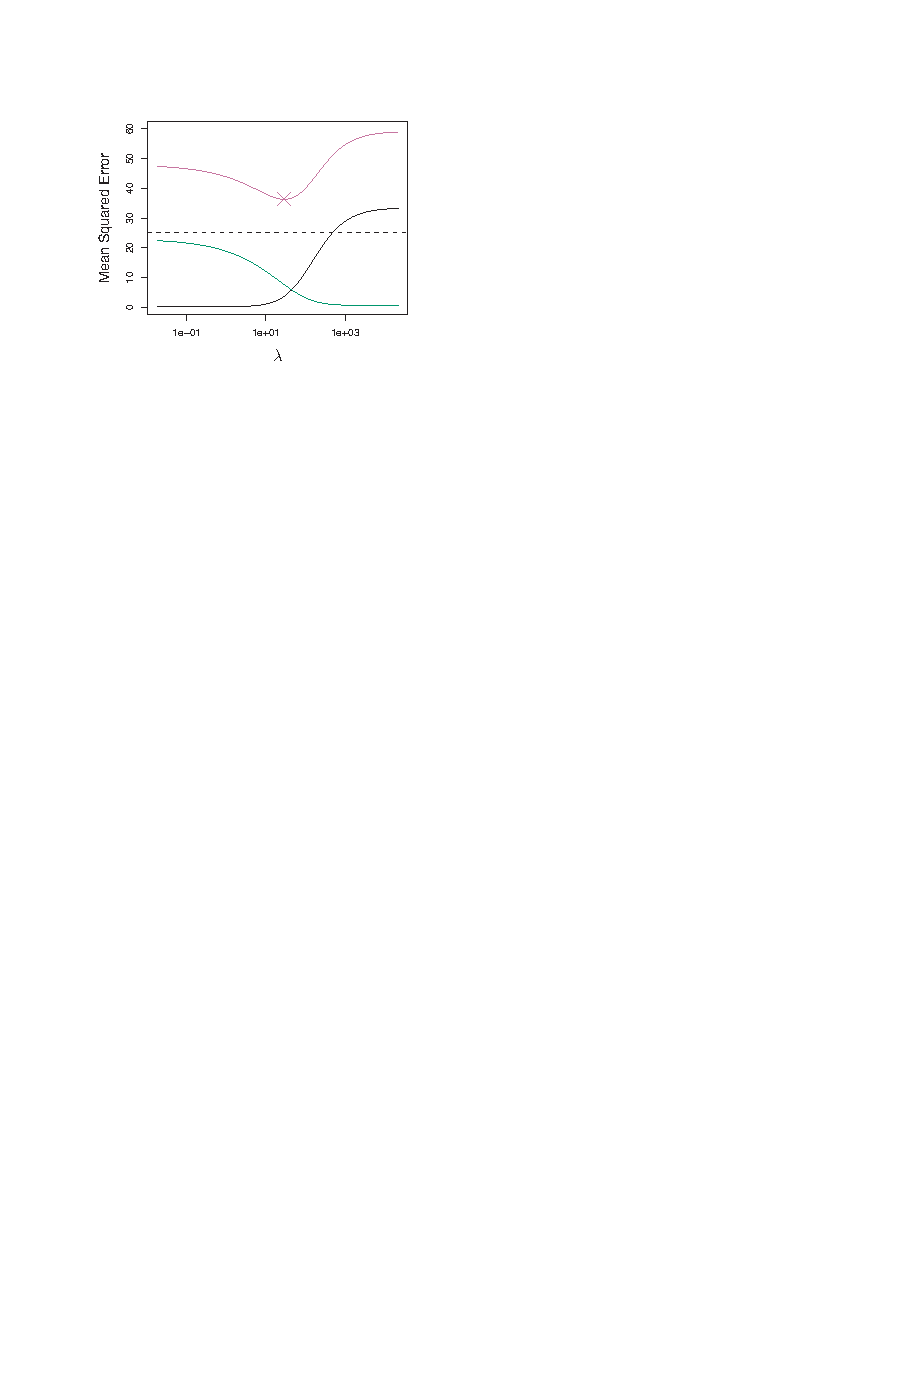
\includegraphics[scale=1.1]{bias-variance-ridge}
\end{figure}

\column{0.3\textwidth}

green: variance\\~\\
black: bias\\~\\
red: total error

\end{columns}

...but how can we choose $\lambda$?\\~\\

Stay tuned (not today, though)
\end{frame}

\begin{frame}{Side note:  ``Regularization''}

\textbf{Regularization} Refers to the process of adding a term to the objective function of a problem that 
\begin{itemize}
\item Makes the problem ``well behaved" (easier to solve)
\item Solves a different problem from the one you originally wanted.\\~\\
\end{itemize}

In our case, the sum of squared coefficients in Ridge makes the problem very simple to solve, but we get coefficients that are biased.\\~\\

In forecasting, the reduction in variance outweighs the growth in variance.  But what about inference? \\~\\

\pause

\begin{columns}
\column{0.6\textwidth}

Vapnik:``\textit{Regularization theory was one of the first signs of the existence of intelligent inference}''\\~\\

Why?  You avoid coefficients you shouldn't have considered.

\column{0.4\textwidth}
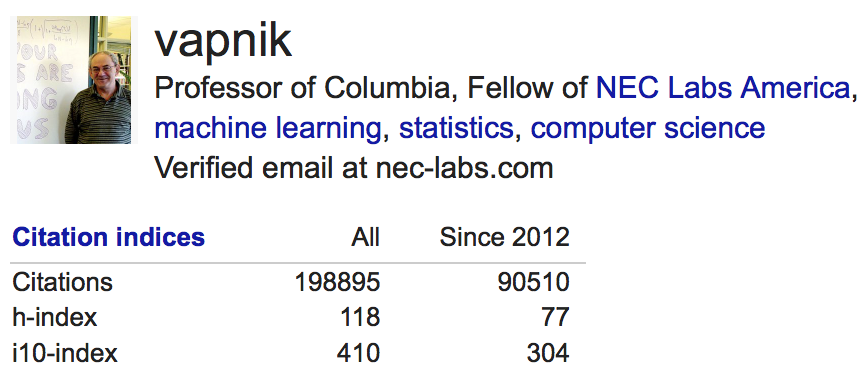
\includegraphics[scale=0.4]{vapnik}
\end{columns}
\end{frame}


\begin{frame}{The Lasso}

“Least Absolute Selection and Shrinkage Operator” (Tibshirani, 1996)\\~\\

Lasso is a simple modification of Ridge:

\begin{align*}
\min_\beta \sum_{i=1}^N \left(Y_i - X_i \beta \right)^2+\lambda \cdot \norm{\beta}_1\text{, where }\norm{\beta}_1=\sum_{k=1}^K |\beta_k|
\end{align*}

Note, we won't find a closed-form expression for the coefficients (unlike ridge and OLS).  Why?

\pause

...Because the $\ell_1$ norm is not differentiable everywhere.

\vspace{5mm}

But you can still use your computer to find the $\hat{\beta}_\text{lasso}$ in a much more efficient way than subset selection.  

\end{frame}

\begin{frame}{Lasso tradeoffs vs OLS, subset selection and ridge regression}

\pause

\begin{enumerate}
\item[$+$] Lasso is faster to solve than subset selection
\item[$-$] Lasso is slower to solve than ridge (no analytic solution)
\item[$+$] Lasso drives parameters to zero, like subset selection and unlike ridge
\begin{itemize}
\item $\Rightarrow$ interpretability
\item But if there really are a lot of modest sized $\beta$, this is undesirable!
\end{itemize}
\item[$-$] Lasso yields biased parameters (unlike OLS / subset selection)
\item[$\pm$] Lasso similar to ridge's prediction bias-variance properties 
\begin{itemize}
\item[$+$] less prediction variance than OLS, especially with many  predictors 
\item[$-$] more prediction bias than OLS
\end{itemize}
\item[$-$] With highly correlated predictors, Lasso is unstable: indifferent between 
\begin{itemize}
\item $\hat{\beta}_1=0$ and $\hat{\beta}_2= \beta_1+\beta_2$
\item $\hat{\beta}_1= \beta_1+\beta_2$ and $\hat{\beta}_2=0$
\end{itemize}
\end{enumerate}

\end{frame}

\begin{frame}{A bit of intuition about what Lasso and ridge are doing}
\begin{columns}
\column{0.25\textwidth}
Each line is a ``contour'' for either the RSS or the regularizing penalties\\~\\

Solutions happen when the contours are tangent to each other
\column{0.7\textwidth}
\begin{figure}
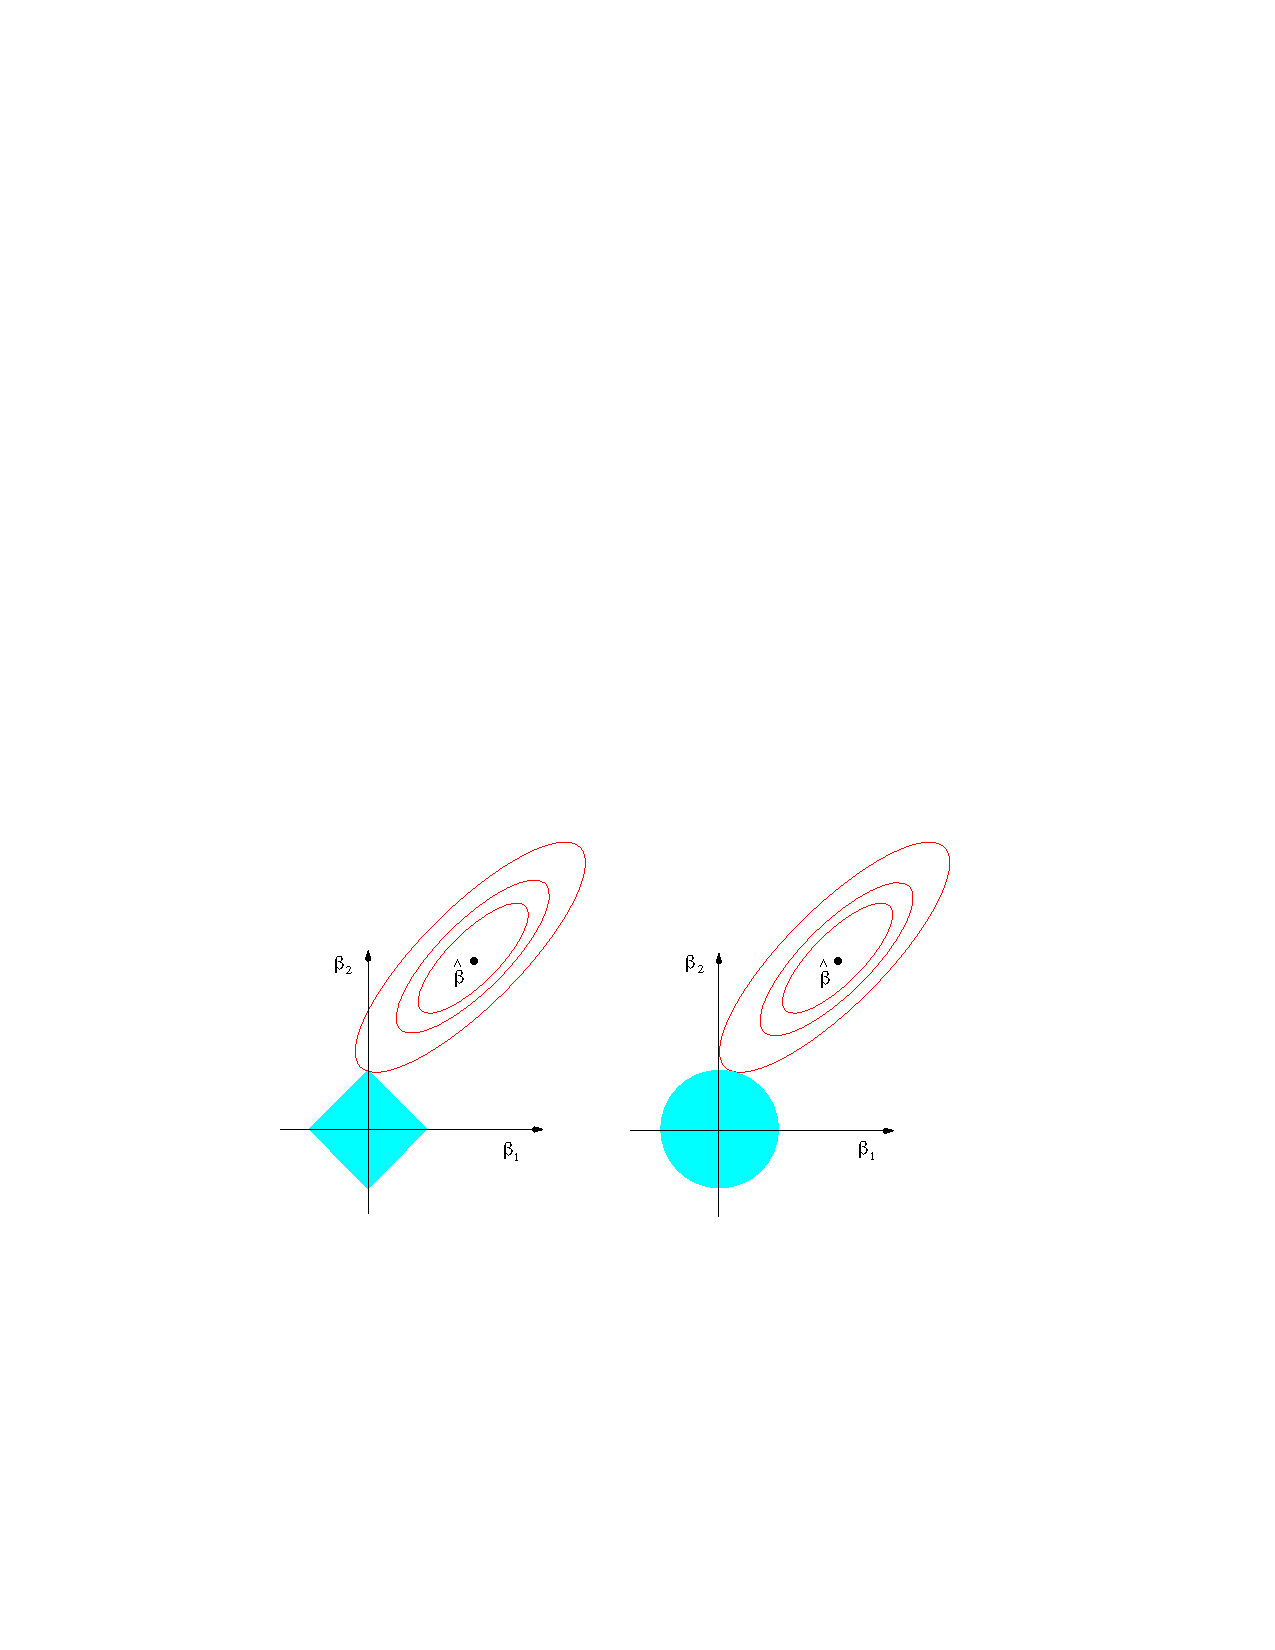
\includegraphics[scale=0.6]{lasso_v_ridge}
\caption*{\tiny Figure taken from Imbens 2015 NBER lecture}
\end{figure}
\end{columns}

\vspace{5mm}

For lasso, you can see this is much more likely to happen at a corner (one parameter zero) than it is for ridge
\end{frame}


\begin{frame}{Supplemental slides}

\end{frame}


\begin{frame}{$C_p$, AIC, BIC or ``Adjusted $R^2$''}

\begin{center}
\begin{tabular}{cc}
Metric & Formula\\
\hline\hline\\
$C_p$ & $\frac{1}{n}\left(RSS + 2d\hat{\sigma}^2\right)$\\\\
AIC & $\frac{1}{n\hat{\sigma}^2}\left(RSS + 2d\hat{\sigma}^2\right)$\\\\
BIC & $\frac{1}{n\hat{\sigma}^2}\left(RSS + \log{(n)}d\hat{\sigma}^2\right)$\\\\
Adjusted $R^2$ & $1-\frac{RSS}{TSS}\frac{(n-1)}{(n-d-1)}$\\\\
\hline
\end{tabular}\\~\\
\end{center}

...where $d$ is the number of predictors and $\hat{\sigma}^2$ is your best estimate of the variance of the model error\\~\\

Note that Adjusted $R^2$ is related to the F-statistic but not the same, and that we don't \textit{always} have $0<\text{Adjusted }R^2<1$

\end{frame}

\begin{frame}{Which error adjustment to use?}

The answer is somewhat a matter of personal taste.

\begin{itemize}
\item $C_p$ and AIC are effectively the same.

\item BIC penalizes added features more than $C_p$ and AIC.

\item $C_p$, AIC and BIC have rigorous derivations.

\item $R^2$ does not have a derivation but it has an intuitive interpretation.\\~\\
\end{itemize}

My two cents:
\begin{enumerate}
\item Look at both AIC and BIC and make a judgment call if they differ
\item Use Adjusted $R^2$ if you want readers to understand the numeric value
\item But if you can afford the computing time, use cross validation instead.
\end{enumerate}
\end{frame}

\end{document}
